\documentclass{article}
\usepackage[utf8]{inputenc}
\usepackage{tikz}
\renewcommand{\thesubsection}{\thesection.\alph{subsection}}
\setlength{\parindent}{0cm}

\title{CS325 Homework 5}
\author{Joshua Barringer \\
        Prof. Schutfort}
\date{5 March 2020}

\begin{document}

\maketitle

\section{}

\subsection{If $Y$ is NP-complete then so is $X$.}

\textbf{False}

We do not know what time category $X$ is in, but we know $Y$ is NP-complete.  $X$ reducing to $Y$ means that $X$ cannot be more difficult than $Y$.  We know $Y$ is difficult, but $X$ reducing to $Y$ doesn't give us enough information to conclude anything about $X$.

\subsection{If $X$ is NP-complete then so is $Y$.}

\textbf{False}

This is not guaranteed because $Y$ is not guaranteed to be in NP.  If $Y$ is in P, and $X$ reduces to $Y$, then NP = P, and all NP problems are polynomial.  Since this has not been disproven, $Y$ must be in NP for this to be true.

\subsection{If $Y$ is NP-complete and $X$ is in NP then $X$ is NP-complete.}

\textbf{False}

Similarly to problem 1.a, there's not enough information to guarantee that $X$ is NP-complete.  If all problems in NP reduce to $Y$, and $X$ reduces to $Y$, then we still don't know whether all problems in NP reduce to $X$.

\subsection{If $X$ is NP-complete and $Y$ is in NP then $Y$ is NP-complete.}

\textbf{True}

If $X$ reduces into $Y$ in polynomial time, then $X$ cannot be more than a polynomial factor harder than $Y$.  Because every problem in NP reduces to an NP-complete problem, every problem in NP reduces to $X$.  Because $X$ can be reduced to $Y$, every problem in NP can be reduced to $Y$.  Therefore, $Y$ must be NP-complete

\subsection{If $X$ is in P, then $Y$ is in P.}

\textbf{False}

If $X$ is in P, then $Y$ is not guaranteed to be in P.  $X$ reducing to $Y$ means that $X$ is no more difficult than $Y$ is, but it can be easier.  $X$ reducing to $Y$ does not mean that $Y$ can reduce to $X$, so we cannot conclude anything about $Y$ if we know that $X$ is in P.

\subsection{If $Y$ is in P, then $X$ is in P}

\textbf{True}

If we can solve $Y$ efficiently, then since $X$ reduces to $Y$ in polynomial time, we use $Y$ to solve $X$ efficiently.  If $Y$ can be solved in polynomial time, it follows that $X$ must be solveable in polynomial time, given that $X$ reduces to $Y$ in polynomial time.

\subsection{$X$ and $Y$ can't both be in NP.}

\section{}

If \textsc{Ham-Cycle} reduces to \textsc{Ham-Path} in polynomial time, \textsc{Ham-Path} is in NP, and \textsc{Ham-Cycle} is NP-Complete, then it follows that \textsc{Ham-Path} is NP-complete.  To show that \textsc{Ham-Path} is NP-complete, we need to do two things:

\begin{itemize}
    \item First, we must show that \textsc{Ham-Path} is in NP
    \item Second, we must show that we can reduce \textsc{Ham-Cycle} to \textsc{Ham-Path} in polynomial time
\end{itemize}

Doing this will satisfy the proof that \textsc{Ham-Path} is NP-complete.

\subsection{}

If we are given a set of edges, $E$, and a graph, $G$, then we can easily determine if the edges complete a Hamiltonian Path in polynomial time.  To show \textsc{Ham-Path} is in NP, we have to verify the path given.  We will start by finding an edge that shares a vertex with only one other edge; this means that it is either a start or end of the Hamiltonian path.  We now check if the path is Hamiltonian by iterating through the list of edges by related vertex.  If we encounter a vertex we've seen before, then we return no.  If we reach the end of the edge list without traveling to every vertex, then we return no.  If we reach the end of the edge list and every vertex has been visited, then we return yes.\\

This will run in polynomial time, because finding the start of the Hamiltonian path will take at max n-1 iterations, and determining the validity of the path will take at max $n$ iterations.  The running time for this algorithm should be $T = O(n)$, which means that \textsc{Ham-Path} is in NP\\

\textsc{Ham-Path(G[], E[])}

\begin{verbatim}
    1  loc = 0
    2  index = 0
    3  while(start-not-found)
    4      if(E[index] has only 1 shared vertex)
    5          loc = index
    6  while(for int i = 0; i < E.length(); i ++)
    7      if(E[loc].visited = false)
    8          E[loc].visited = true
    9      else
    10         return false
    11     loc = next edge
    12 if(all-vertices-have-been-visited)
    13     return true
    14 else
    15     return false
\end{verbatim}

\subsection{}

Next, we have to show that \textsc{Ham-Cycle} can be reduced to \textsc{Ham-Path} in polynomial time.  Transforming a \textsc{Ham-Cycle} graph into a \textsc{Ham-Path} graph is a very simple task.  We take any vertex, $v$, in the \textsc{Ham-Cycle} graph, $G$, and duplicate it to create $v'$.  $v'$ has an edge connecting itself to every vertex that $v$ is connected to.  This is a short operation and can easily be done in at least polynomial time.  Once we have done this, the Hamiltonian Cycle validity can be decided the same way we do the Hamiltonian path.  If there exists a Hamiltonian path between $v$ and $v'$, then a Hamiltonian Cycle exists.\\

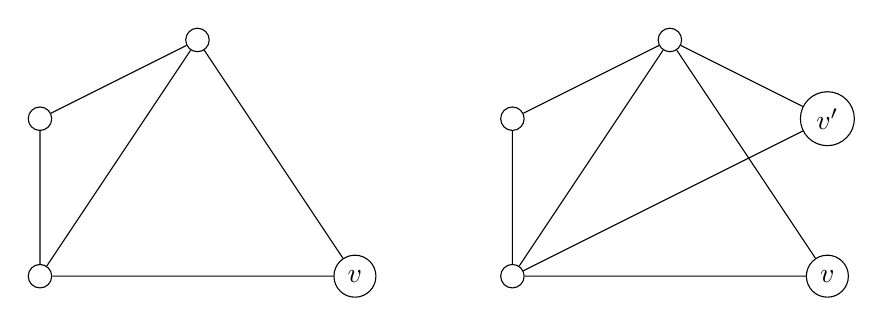
\begin{tikzpicture}[every node/.style={circle,draw = black, inner sep=3pt, fill=white},]
  \node (A) at (0,0) {};
  \node (B) at (0,2) {};
  \node (C) at (2,3) {};
  \node (D) at (4,0) {$v$};
  
  \node (a) at (6,0) {};
  \node (b) at (6,2) {};
  \node (c) at (8,3) {};
  \node (d) at (10,0) {$v$};
  \node (e) at (10,2) {$v'$};
  
  \draw (a) -- (b)
        (b) -- (c)
        (a) -- (c)
        (c) -- (d)
        (a) -- (d)
        (c) -- (e)
        (a) -- (e);
  
  \draw (A) -- (B)
        (B) -- (C)
        (A) -- (C)
        (C) -- (D)
        (A) -- (D);
\end{tikzpicture}

We have shown that \textsc{Ham-Path} is in NP, and \textsc{Ham-Cycle} can be reduced to \textsc{Ham-Path} in polynomial time. It must be true, given that \textsc{Ham-Cycle} is NP-complete, that \textsc{Ham-Path} is NP-complete as well.

\section{}

\subsection{}

We can determine if a graph has 2-coloring by using a breadth-first-search through the graph, and assigning alternating colors at each increment of distance from our source vertex.  If, during BFS, we encounter a visited node with the same color as our current node, then the 2-coloring fails.  For this algorithm, we use an int, $c$, to determine the color and visit status simultaneously.  A $c$ value of 0 is unvisited, $c = 1$ is color 1, and $c = 2$ is color 2.

\textsc{2-Color(G[])}

\begin{verbatim}
    1  c=1
    2  queue = [G[0]]
    3  source = queue[0]
    4  while(queue is not empty):
    5      for each item in queue:
    6          source.color = c
    7          for each child node of source:
    8              if child.color < 0:
    9                  queue.append(child node)
    10             else if child.color == source.color
    11                 return false
    12     
    13     if(c == 1)
    14         c = 2
    15     else
    16         c = 1
    17 return true
\end{verbatim}

This code only visits each vertex of the graph once, so the running time will be $T = O(V)$.

\subsection{}

To show that 4-Color is NP-complete, we need to show:

\begin{itemize}
    \item 4-Color is in NP
    \item 3-Color reduces to 4-Color in polynomial time
\end{itemize}

\subsubsection{}

4-Color is in NP because we can determine the validity of a decision problem in polynomial time.  Given a possible solution to a 4-Color graph, $G$, we iterate through each edge in $E$.  If every edge has vertices of different colors, then we return true.  If we encounter an edge whose vertices share the same color, then we return false.  Since we're only checking each vertex one time, we can complete this problem in polynomial time.  It follows that 4-Color is in NP.

\subsubsection{}

We can reduce 3-Color to 4-Color by using the graph, $G$, for 3-Color, a copy of $G$, $G'$, for 4-Color.  We will add a new vertex with the 4th color, $a$, to $G'$, where $a$ is connected to every single other vertex in $G'$.  Since $a$ is the only graph in $G'$ that is the fourth color, if the 4-Color decision problem returns true, then the we know that $G$ passes 3-Color.  Conversely, if we have a 3-Color graph, $G$, that we know is a correct 3-Color, then the corresponding reduction to 4-Color, $G'$, will be a correct 4-Color graph.\\

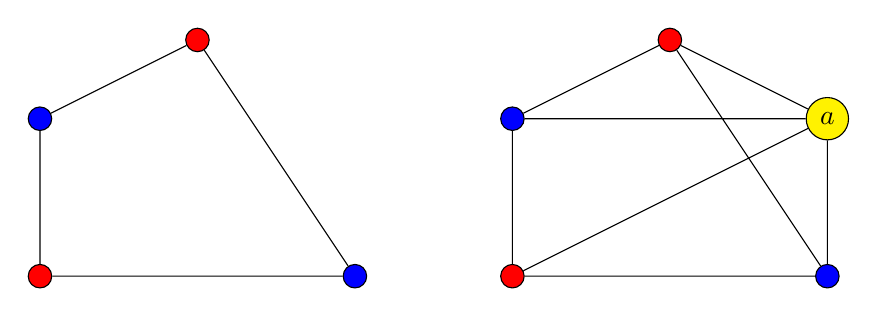
\begin{tikzpicture}[
red/.style={circle,draw = black, inner sep=3pt, fill=red},
blue/.style={circle,draw = black, inner sep=3pt, fill=blue},
green/.style={circle, draw=black, inner sep=3pt, fill=yellow}
]
  \node[red] (A) at (0,0) {};
  \node[blue] (B) at (0,2) {};
  \node[red] (C) at (2,3) {};
  \node[blue] (D) at (4,0) {};
  
  \node[red] (a) at (6,0) {};
  \node[blue] (b) at (6,2) {};
  \node[red] (c) at (8,3) {};
  \node[blue] (d) at (10,0) {};
  \node[green] (e) at (10,2) {$a$};
  
  \draw (A) -- (B)
        (B) -- (C)
        (C) -- (D)
        (A) -- (D);
            
  \draw (a) -- (b)
        (b) -- (c)
        (c) -- (d)
        (a) -- (d)
        (a) -- (e)
        (b) -- (e)
        (c) -- (e)
        (d) -- (e);
\end{tikzpicture}

Because we have shown that 4-Color is in NP, and 3-Color reduces to 4-Color in polynomial time, we can conclude that 4-Color is NP-Complete.

\end{document}
